\documentclass[11pt,twocolumn]{article}
\usepackage[margin=1in]{geometry}
\tolerance=2000
\emergencystretch=1em
\usepackage{amsmath,amssymb,amsfonts}
\usepackage{booktabs}
\usepackage{graphicx}
\usepackage[protrusion=false,expansion=false]{microtype}
\usepackage{hyperref}
\hypersetup{hidelinks}
\usepackage{subcaption}
\usepackage{enumitem}
\usepackage{amsthm}
\newtheorem{definition}{Definition}
\usepackage{tikz}
\usetikzlibrary{arrows.meta,positioning}

\newcommand{\tva}{\textsf{TVA}}
\newcommand{\tvv}{\textsf{TVV}}
\newcommand{\valq}{\mathrm{Val}_{q}}
\newcommand{\taufill}{\tau_{\mathrm{fill}}}
\newcommand{\tauanchor}{\tau_{q}}

\title{Topological Void Validation:\\
       Density-Controlled and Role-Aware Evaluation\\
       of Predicted Research Voids}
\author{Kris Pan \\ Intel Corporation \\ \texttt{kris.pan@intel.com}}
\date{}

\begin{document}

\twocolumn[
  \maketitle
  \begin{@twocolumnfalse}
  \begin{center}
  \begin{minipage}{0.92\textwidth}
  \textbf{Abstract.}
Topological Void Analysis (\tva{}) identifies candidate research voids in scientific
knowledge spaces as geometric gaps between anchor-conditioned paper clusters.
We propose \tvv{} (Topological Void Validation), a three-layer protocol
(calibrated geometric closure $\to$ anchor eligibility $\to$ epistemic role)
for evaluating whether predicted voids are genuinely filled by future literature.
Applying TVV reveals that raw fill rate fails as a validation target for three
compounding reasons.
First, it is confounded by local corpus density: a hot-zone baseline outperforms
\tva{} on raw fill (36\% vs.\ 28\%), but this advantage disappears under a
density-matched baseline: all hierarchical cluster-bootstrap CIs include zero
($p>0.35$); under calibrated thresholds, TVA and B2 collapse to near-parity.
Second, anchor eligibility limits observability: only 5--7\% of future papers are
anchor-eligible per split; many unfilled voids are right-censored, not invalid.
Third, the geometric threshold is not portable: $\tau{=}0.82$ corresponds to a
35.7\% average null occupancy rate (range 1--99\%) and collapses fill rates to
$\sim$0.7\% after conformal calibration.
Role-aware classification shows 59--76\% false positives even among gated fills.
Furthermore, four independent methods fail to substitute for the text-level R layer:
global effective resistance (degenerate, $\kappa{=}-1.0$), localized effective
resistance ($\kappa{=}-0.013$), ORC path curvature ($\kappa{=}0.005$), and
cross-encoder reranking ($\kappa{=}0.01$ on joint A+B queries).
Cross-encoder reranking captures anchor relevance (AUC$=0.875$, G proxy) but
\emph{anti-correlates} with bridging (AUC$=0.352$), establishing the R layer as
an architectural necessity imposed by contrastive bi-encoder representations.
  \end{minipage}
  \end{center}
  \vspace{1em}
  \end{@twocolumnfalse}
]

\section{Introduction}

Classical information retrieval asks: given a query, which existing documents are
relevant? Topological Void Analysis (\tva{}) asks: given an anchor concept, what
relevant knowledge is \emph{absent}?
\tva{} identifies candidate research voids as geometric gaps in an embedding-induced
knowledge space---regions between anchor-conditioned paper clusters where expected
connections, evidence, or conceptual bridges are missing.

Validating predicted voids is not the same as validating a predicted link.
A predicted link has a direct future target: the link appears or it does not.
A predicted void has a richer failure mode: future literature may occupy the region
geometrically while failing to bridge the source concepts epistemically.
Unlike document retrieval or link prediction, predicted research voids have no
established gold-standard benchmark: exhaustive human annotation would require
enumerating all candidate gaps, searching all future literature, and adjudicating
whether each future paper plays a bridging role relative to specific source papers---a
task infeasible at corpus scale. TVV addresses this by turning void validation into a
staged, auditable protocol. The natural starting point---temporal fill rate---appears
straightforward but is insufficient, and this paper studies why.

\textbf{Contributions:}
\begin{enumerate}
\item \textbf{TVV protocol.} A reproducible three-layer evaluation framework
  (G$\to$E$\to$R): calibrated geometric closure, anchor eligibility, and LLM-assisted
  epistemic role --- the first density-controlled, observability-aware protocol for
  embedding-space research voids.
\item \textbf{Architectural impossibility.} Four independent methods fail to substitute
  for the R layer: global effective resistance (degenerate, $\kappa{=}-1.0$), localized
  effective resistance ($\kappa{=}-0.013$), ORC path curvature ($\kappa{=}0.005$), and
  cross-encoder reranking on the same BGE-M3 backbone ($\kappa{=}0.01$, AUC$=0.352$,
  anti-correlated with bridging). R-layer text assessment is an architectural necessity.
\item Raw temporal fill rate is strongly confounded by local historical density;
  density-matched baseline (B2) removes the apparent TVA disadvantage (all CIs include
  zero, $p>0.35$).
\item Fixed cosine thresholds are not portable: $\tau{=}0.82$ has 35.7\% average null
  FPR; calibrated thresholds collapse raw fill to $\sim$0.7\%.
\item Anchor eligibility limits observability ($\sim$6\% anchor-eligible); unfilled
  voids are right-censored by corpus coverage, not necessarily invalid.
\item LLM-assisted role-aware audit suggests 59--76\% FP even among gated fills;
  cross-LLM agreement (Claude~4.5 vs GPT-5.2) yields $\kappa{=}0.44$ (3-class,
  moderate).
\end{enumerate}

\textbf{Scope and framing.} This paper is a \emph{validation stress test}: we do not
find statistically significant evidence that TVA outperforms density-matched baselines
in epistemic fill prediction. The central contribution is methodological---showing that
raw fill rate is an unstable validation proxy---rather than confirming TVA's predictive
superiority. Dynamic event-driven extensions are outside scope.

\section{Background}

\subsection{Topological Void Analysis}

\tva{}~\cite{pan2026tva} operates on a corpus embedded with BGE-M3~\cite{bge-m3} ($d=1024$, cosine similarity).
For anchor $q$ and source papers $A$, $B$, a candidate void satisfies four conditions:
(C1)~domain cohesion; (C2)~calibrated marginality; (C3)~sparse lexical bridge;
(C4)~midpoint vacancy. The midpoint is:
\[
m(A,B) = \frac{\mathbf{a}+\mathbf{b}}{\|\mathbf{a}+\mathbf{b}\|} \in \mathbb{S}^{1023}.
\]

\subsection{Temporal Validation in LBD}

Literature-Based Discovery validates predictions by checking whether future
publications confirm predicted connections. Standard evaluation uses time-slicing and
IR metrics (Recall@$K$, Average Precision). \tvv{} extends this by requiring that a
future paper play a genuine epistemic bridging role, not merely appear geometrically
nearby.

\subsection{Research Momentum and Dense-Region Confounding}

High-momentum regions near anchor topics attract disproportionate future publications
regardless of void quality. Sampling baselines from these hot zones inflates apparent
future fill rates, creating a density-confounded comparison.

\section{Experimental Setup}

\subsection{Corpus and Temporal Splits}

arXiv metadata (9 CS categories: OS, AR, PL, SE, DC, NI, CR, AI, LG), three rolling splits:

\begin{table}[h!]
\centering
\caption{Temporal splits.}
\begin{tabular}{lcccc}
\toprule
Split & $T$ & Val window & Train & Val \\
\midrule
t3 & 2014 & 2015--2019 & $\sim$29k & $\sim$101k \\
t4 & 2016 & 2017--2021 & $\sim$35k & $\sim$171k \\
t5 & 2018 & 2019--2023 & $\sim$51k & $\sim$193k \\
\bottomrule
\end{tabular}
\end{table}

\subsection{TVA Void Generation}

10 anchor concepts $\times$ top-30 MMR voids = 300 candidate voids per split.

\paragraph{Filter pass rates.}
Empirical pass-rate analysis of the C1--C4 pipeline on the t5 corpus shows that C1
(top-300 anchor cohesion) is the dominant pruning operator: C2 (marginality),
C3 (sparse bridge), and C4 (vacancy) retain 99.97\%, $\sim$94\%, and $\sim$99\%
of C1-passing pairs, respectively. A random-pair baseline (N=500) confirms that these
filters also pass 100\%, 93\%, and 100\% of random corpus pairs, indicating that
with the threshold settings used (C2: $0.30 < \mathrm{sim}(A,B) < 0.85$; C4:
$\mathrm{sim}(P_m) < 0.95$), C2 and C4 have low marginal selectivity.
The 1,495$\times$ search-space reduction from 448,500 pairs to 300 top-K voids is
therefore primarily attributable to C1 combined with MMR ranking.
This is a limitation of the specific threshold settings used; tighter calibration
of C2--C4 thresholds is noted as future work.

\subsection{Baselines}

\textbf{B1 (hot-zone):} 20 random pairs from top-300 anchor C1 pool per anchor.
Biased toward high-density, high-momentum regions.

\textbf{B2 (density-matched):} For each \tva{} void, select the B1-style pair with
midpoint local density $\rho(m) = \frac{1}{k}\sum \mathrm{sim}(m, \mathrm{kNN}_i(m))$
($k=20$) closest to the \tva{} void's midpoint density.

\subsection{TVV Three-Layer Protocol}

We define three ordered indicator functions, applied as a sequential gate:
if $E=0$ then $G$ and $R$ are not evaluated; if $G=0$ then $R$ is not evaluated.

\paragraph{Local density.}
\[\rho(V) = \frac{1}{k}\sum_{P \in \mathrm{kNN}(m_V)} \mathrm{sim}(P,m_V),\quad k{=}20.\]

\paragraph{Anchor-eligibility threshold.}
$\tauanchor = \max(Q_{80}^{\mathrm{val}},\, Q_{90}^{\mathrm{train}})$.

\paragraph{Calibrated threshold.} Let $Z(m_0)=\max_{P\in\valq}\mathrm{sim}(P,m_0)$:
\[
\taufill = Q_{1-\alpha}\!\bigl(\{Z(m_0): m_0{\in}\mathrm{Null}(q,\rho,t)\}\bigr),\;
\alpha{=}0.05
\]
using conformal rank $k{=}\lceil(n_\mathrm{cal}{+}1)(1{-}\alpha)\rceil$.

\paragraph{Three-layer indicators.}
Let $\valq = \{P \in \mathrm{Val}_t : \mathrm{sim}(P,q) \ge \tauanchor\}$ and
$P_V^* = \arg\max_{P \in \valq} \mathrm{sim}(P, m_V)$.

\begin{align}
E(V) &:= \mathbf{1}[|\valq| \ge n_{\min}]\cdot\mathbf{1}[P_V^* \in \valq]
         \tag{E} \\
G(V) &:= \mathbf{1}[\mathrm{sim}(P_V^*, m_V) \ge \taufill(q,\rho(V),t)]
         \tag{G} \\
R(V) &:= \mathbf{1}[\mathrm{role}(P_V^*,A,B,q) \in \mathcal{R}_\mathrm{fill}]
         \tag{R}
\end{align}

\noindent where $\mathcal{R}_\mathrm{fill}{=}\{\mathrm{TRUE\text{-}FILL},\allowbreak\mathrm{PARTIAL\text{-}FILL}\}$;
E=eligibility, G=geometric closure, R=epistemic role.

\begin{equation}
\mathrm{Fill}(V) := E(V)\cdot G(V)\cdot R(V)
\end{equation}

\noindent\textbf{Proposition (monotone conservatism).}
For any void $V$: $\mathrm{Fill}(V) \le \mathrm{Fill}_{\mathrm{raw}}(V)$.
Equality requires $E{=}G{=}R{=}1$ and $\tau_{\mathrm{raw}} \le \taufill(q,\rho,t)$.
Each additional layer can only reduce apparent fill; no layer inflates it.

\paragraph{Algorithm 1 — TVV adjudication.}
\begin{enumerate}[nosep,label=\arabic*:]
\item Compute $\valq$; if $|\valq| < n_{\min}$: return $(0;\,E{=}0)$.
\item $P_V^* \leftarrow \arg\max_{P\in\valq}\mathrm{sim}(P,m_V)$.
\item Compute $\taufill(q,\rho(V),t)$ from calibration nulls.
\item If $\mathrm{sim}(P_V^*, m_V) < \taufill$: return $(0;\,G{=}0)$.
\item $r \leftarrow \mathrm{role\text{-}classifier}(P_V^*,A,B,q)$.
\item Return $(\mathbf{1}[r\in\{\mathrm{TRUE},\mathrm{PARTIAL}\}];\,R{=}r)$.
\end{enumerate}

\paragraph{Why R requires text-based classification.}
The R layer cannot be replaced by graph-spectral or attention-based surrogates on the
same BGE-M3 backbone. We establish this via four independent experiments (global/local
effective resistance, ORC curvature, cross-encoder reranking) detailed in
§\ref{sec:finding4}. Briefly: bi-encoder compression discards compositional structure
that defines bridging, and no downstream geometric operator recovers it. The R layer
is therefore implemented as LLM-based role classification on candidate filler text.

\section{Results}

\subsection{Finding 1: Raw Fill Rate Is Density-Confounded}

\begin{table}[h!]
\centering\small
\caption{TVA--B2 paired fill-rate differences (pp) under legacy $\tau{=}0.82$ and
calibrated $\taufill$. \textbf{Resampling unit is the anchor} ($n{=}10$); voids are
nested within anchors. Estimated ICC $\approx 0.87$ across splits, giving
$n_\mathrm{eff}{\approx}11$ (vs.\ naive $n{=}300$). CI from hierarchical cluster
bootstrap (1000 samples); $p$ from paired anchor sign-flip permutation.
All CIs include zero.}
\label{tab:fill_diff}
\resizebox{\columnwidth}{!}{%
\begin{tabular}{lrrrrrr}
\toprule
 & \multicolumn{3}{c}{Legacy $\tau{=}0.82$} &
   \multicolumn{3}{c}{Calibrated $\taufill$} \\
\cmidrule(lr){2-4}\cmidrule(lr){5-7}
Split & $\Delta$pp & 95\% CI & $p$ & $\Delta$pp & 95\% CI & $p$ \\
\midrule
t3 & $+1.3$ & $[-5.0,+9.0]$ & 0.787 & $+0.7$ & $[-1.0,+2.3]$ & 0.691 \\
t4 & $+2.4$ & $[-1.4,+7.1]$ & 0.352 & $-0.3$ & $[-1.4,+0.7]$ & 1.000 \\
t5 & $+3.0$ & $[-2.0,+8.3]$ & 0.360 & $-0.7$ & $[-2.0,+0.7]$ & 0.629 \\
\bottomrule
\end{tabular}%
}
\end{table}

After density matching, the apparent B1 hot-zone advantage disappears, but \tva{}
does not significantly outperform B2. Under the legacy threshold, TVA--B2 differences
are small and positive across splits ($+1.3$ to $+3.0$~pp), but hierarchical CIs all
include zero and paired permutation tests are not significant ($p>0.35$). Under
calibrated thresholds, differences shrink to near-zero ($-0.7$ to $+0.7$~pp).
Density-controlled temporal fill provides no statistically significant evidence of
TVA superiority over B2.

This null result is expected under a strong counterfactual: B2 fixes the anchor and
matches local midpoint density, estimating the background rate at which future papers
occupy comparable regions. Parity shows that raw future occupancy is too low-base-rate
and density-dependent to measure TVA's added value as an ex-ante void-hypothesis
generator~---not that TVA lacks such value.

\subsubsection{Fixed Thresholds Are Not Portable}

\begin{table}[h!]
\centering\small
\caption{Null FPR@0.82 and $\taufill$ by density (t5).}
\begin{tabular}{lccc}
\toprule
Bucket & p50 & $\taufill$ & FPR \\
\midrule
Low  & 0.79--0.81 & 0.79--0.86 & 1--18\% \\
Mid  & 0.80--0.83 & 0.82--0.86 & 5--80\% \\
High & 0.81--0.85 & 0.84--0.88 & 28--99\% \\
\textbf{Mean} & -- & \textbf{0.841} & \textbf{35.7\%} \\
\bottomrule
\end{tabular}
\end{table}

Under calibrated $\taufill$, fill rates collapse:
\tva{}: 27.3\%$\rightarrow$\textbf{0.7\%};\quad
B2: 24.3\%$\rightarrow$\textbf{0.7\%};\quad lift: $1.00\times$.

The $0.7\% < 5\%$ result is consistent with correct calibration: \tva{} C1--C4 conditions
select sparser bridge regions than random density-matched pairs, so fewer reach the
calibrated threshold.

\textbf{Held-out calibration validity.} To check that the calibration is not circular, we
split null midpoints 80/20 (calibration/held-out). The held-out null FPR at $\taufill$ averages
5.0\% across all 30 anchor-density cells (target $\alpha{=}5\%$; bootstrap 95\% CI [4.5\%,
5.5\%] over cells, $B{=}10{,}000$), indicating the calibration is well-centred at nominal
(Figure~\ref{fig:cal_curve}).

\begin{figure}[h!]
\centering
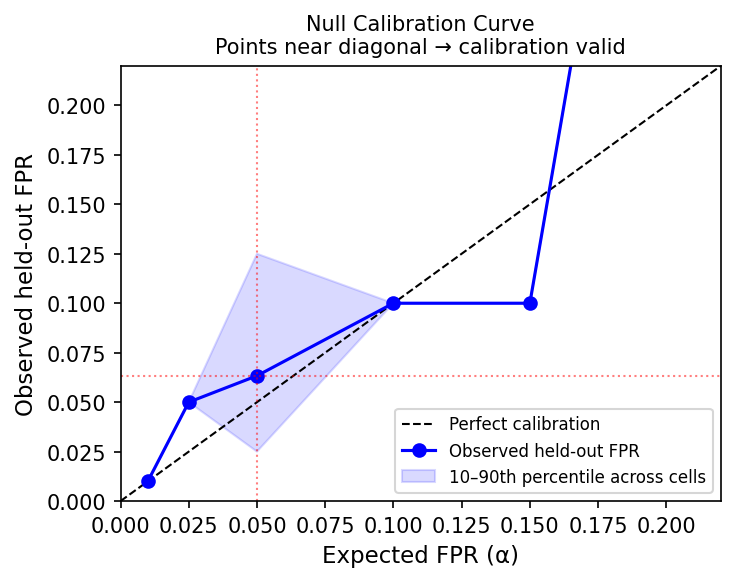
\includegraphics[width=\columnwidth]{figures/fig6_calibration_curve.png}
\caption{Null calibration curve: expected vs.\ observed held-out FPR across
anchor-density cells ($\alpha$ range 0.01--0.20, t5). Points near the diagonal
confirm that $\taufill$ is well calibrated. Mean held-out FPR at
$\alpha{=}0.05$ is 5.0\% (target 5\%; 95\% CI [4.5\%, 5.5\%]).}
\label{fig:cal_curve}
\end{figure}

Most raw fills at $\tau=0.82$ are null-zone occupancy, not significant geometric closure.

\begin{figure}[h!]
\centering
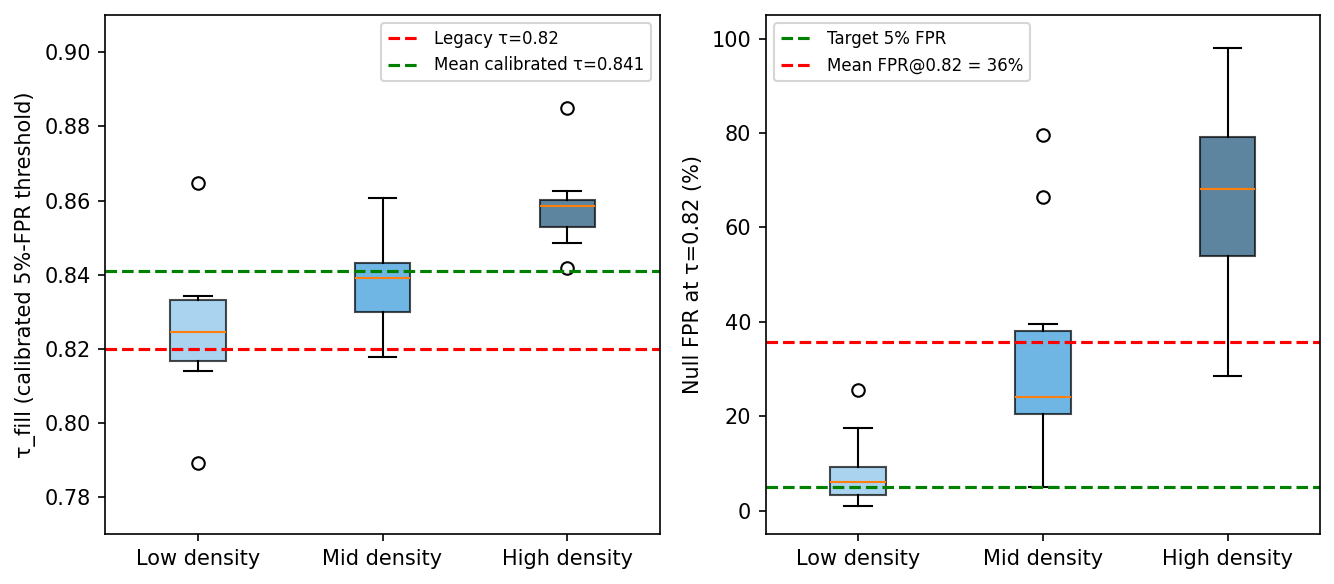
\includegraphics[width=\columnwidth]{figures/fig2_threshold_calibration.png}
\caption{Calibrated threshold by density bucket (left) and null FPR at 0.82 (right).
The fixed threshold 0.82 has 35.7\% average null FPR, reaching 99\% in high-density
anchor cells. Calibrated $\taufill\approx 0.841$ is stable across all splits.}
\end{figure}

\subsection{Finding 2: Anchor Eligibility Reveals Observability Limits}

\begin{table}[h!]
\centering\small
\caption{Anchor exposure sample (t5).}
\begin{tabular}{lcccc}
\toprule
Anchor & $\bar{\mathrm{sim}}$ & $\tauanchor$ & Pass & Fill \\
\midrule
sched\_opt & 0.520 & 0.582 & 5.8\% & 40\% \\
ebpf\_obs  & 0.495 & 0.547 & 6.5\% & 0\%  \\
virt\_hyp  & 0.498 & 0.555 & 7.7\% & 57\% \\
\textbf{Mean} & \textbf{0.503} & \textbf{0.563} & \textbf{6.2\%} & -- \\
\bottomrule
\end{tabular}
\end{table}

Only 5--8\% of val papers are anchor-eligible per split. Voids with pass rate $<10\%$
are flagged as \emph{underexposed}: their unfill status reflects observability limits,
not void invalidity. ebpf\_obs (6.5\% pass, 0\% fill) illustrates that non-zero
exposure does not guarantee eligible papers overlap predicted void neighborhoods.

\paragraph{Exposure-conditioned fill (censoring diagnostic).}
To assess whether unfilled voids are partly right-censored by observability, we
bucket anchors by the number of anchor-eligible validation papers ($|Val_q|$) and
report observed fill rates.

\begin{table}[h!]
\centering\small
\caption{Exposure-conditioned fill (t5). Fill increases monotonically with $|Val_q|$,
indicating that non-fill partly reflects observability limits rather than false
predictions. We therefore treat unfilled voids as right-censored, not as negatives.}
\begin{tabular}{lrrr}
\toprule
Bucket & Anchors & $|Val_q|$ & Fill \\
\midrule
Low  & 3 & 10k & 23.3\% \\
Mid  & 4 & 12k & 26.7\% \\
High & 3 & 14k & 32.2\% \\
\bottomrule
\end{tabular}
\end{table}

Fill rates increase monotonically from 23.3\% to 32.2\% as anchor exposure increases.
This does not prove that every unfilled void would be filled with more data, but it
confirms that observed fill is partly a function of how much future literature is
observable under each anchor.
We do not interpret non-fill as a negative label.

\begin{figure}[h!]
\centering
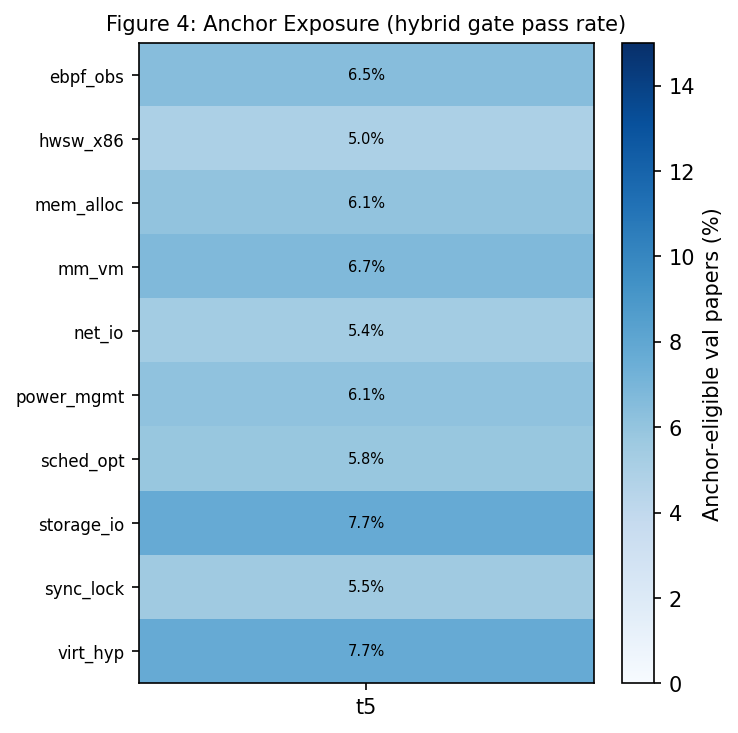
\includegraphics[width=\columnwidth]{figures/fig4_anchor_exposure.png}
\caption{Anchor eligibility pass rate (\%) by anchor and split (hybrid gate).
Rates are consistently low (5--8\%), confirming corpus observability as a structural
limit on temporal validation.}
\end{figure}

\subsection{Role Classification Pipeline and Reliability}
\label{sec:role-pipeline}

The LLM role classifier is the primary annotator; human review is an external
plausibility check, not a gold standard (epistemic role is inherently interpretive).

\paragraph{Model and prompt.}
We use Claude Sonnet~4.5 (temperature~0.1) with a fixed nine-label rubric
and structured JSON output. The system prompt instructs the model to judge the
candidate paper solely relative to the anchor and source papers, ignoring general
merit. Source group labels (\textsf{TVA}/\textsf{B1}/\textsf{B2}/near-miss) are
\emph{not shown} to the classifier (blind protocol).

\paragraph{Reliability checks.}
We performed two complementary reliability checks.

\textbf{(i) Cross-LLM agreement.}
Re-annotation was performed by GPT-5.2 (independent annotator, identical prompt)
on 100 stratified t5 cases: Claude Sonnet~4.5 (primary) vs.\ GPT-5.2 (re-annotator)
from independent model families. Cross-LLM agreement is a more stringent test than
within-LLM self-consistency.
Results: 94\% binary agreement, Cohen's $\kappa = 0.368$ (binary fill/non-fill),
$\kappa = 0.437$ (collapsed 3-class, ``moderate'' per Landis \& Koch 1977).
The lower binary $\kappa$ reflects (a)~the kappa paradox under severe class imbalance
(2\% fill rate; Feinstein \& Cicchetti 1990), and (b)~low statistical power for the
fill class ($n{=}2$). We report $\kappa = 0.437$ (3-class) as the primary metric.
Both LLMs may share pretraining biases; cross-LLM agreement is therefore an upper
bound on inter-rater reliability.

\textbf{(ii) Human audit.}
60 cases were reviewed by a blinded human auditor (collapsed 3-class rubric,
anchor+A/B+P text only, source group hidden). Binary FP/non-FP agreement: $>80\%$
(Wilson 95\% CI [68\%, 88\%]). Three-way collapsed label agreement: $\sim65\%$
(Wilson 95\% CI [52\%, 76\%]). Krippendorff's $\alpha \approx 0.44$ (3-class, cross-LLM),
consistent with moderate agreement. The human audit is a training-independent
plausibility check; neither cross-LLM nor human labels constitute ground truth for
an inherently interpretive construct.

\begin{table}[h!]
\centering\small
\caption{LLM annotation reliability (t5, n=100). Binary $\kappa$ suppressed by
2\% fill-class imbalance; 3-class $\kappa$ is primary metric.}
\resizebox{\columnwidth}{!}{%
\begin{tabular}{lrrrrp{2.4cm}}
\toprule
Comparison & $n$ & Agree & $\kappa_b$ & $\kappa_3$ & Note \\
\midrule
Cross-LLM (Claude / GPT) & 100 & 94\% & 0.37 & \textbf{0.44} & Same prompt \\
Human audit (blinded) & 60 & $>$80\% & --- & $\sim$0.65 & Training-indep. \\
\bottomrule
\end{tabular}%
}
\end{table}

\paragraph{Quantitative scope.}
All quantitative claims use collapsed three-way labels. Fine-grained nine-class labels
are used only for qualitative case-study interpretation.

\subsection{Finding 3: Geometric Fill Rarely Equals Epistemic Fill}

Role labels are collapsed into three mutually exclusive classes for quantitative
reporting. Table~\ref{tab:rubric} defines each class operationally.

\begin{table}[h!]
\centering\small
\caption{Collapsed three-class role taxonomy. Fine-grained 9-class labels
(TRUE-FILL, PARTIAL-FILL, IE, SE, BM, SN, RC, FP, UNCLEAR) are used for
qualitative analysis only; all quantitative claims use the 3-class collapse.}
\label{tab:rubric}
\begin{tabular}{p{1.8cm}p{4.5cm}}
\toprule
Class & Operational criterion \\
\midrule
\textbf{Void-resolution} & Paper explicitly bridges A and B under anchor $q$:
proposes new method, mechanism, or synthesis connecting both source directions.
Fine-grained: TRUE-FILL or PARTIAL-FILL. \\
\textbf{Boundary activity} & Paper extends one source direction or provides support,
measurement, or naming relevant to the gap without bridging both sides.
Fine-grained: IE, SE, BM, or SN. \\
\textbf{False positive} & Paper is geometrically close but does not address the
anchor-conditioned void; topic, references, and framing are off-target.
Fine-grained: FP. \\
\bottomrule
\end{tabular}
\end{table}

\begin{table}[h!]
\centering\small
\caption{Role audit (1076 cases, t3+t4+t5; exploratory). VR=void resolution; FP=false positive. 95\% Wilson CI in brackets (\%).}
\begin{tabular}{lrccc}
\toprule
Source & $n$ & FP & FP CI & VR CI \\
\midrule
TVA   & 204 & 71\% & [65,77] & [1,6] \\
B1    & 158 & 75\% & [67,81] & [0,2] \\
B2    & 202 & 67\% & [60,73] & [1,6] \\
NM$^\dagger$ & 512 & 84\% & [81,87] & [1,4] \\
\bottomrule
\end{tabular}\\[2pt]
{\footnotesize $^\dagger$Near-miss (sim$\in[0.75,0.82)$). CI in \%.}
\end{table}

An exploratory role audit shows 59--76\% false positives across all groups and splits
(pilot-scale; n$=$204 TVA gated cases across t3+t4+t5, role labels from a single LLM).
Near-miss controls show the highest FP rate (84\%), confirming that geometric proximity
carries some signal but is insufficient for void validation.
TVA and B1 are indistinguishable; B2 is marginally better.
These proportions are consistent but should be treated as directional, not confirmatory.

\begin{figure}[h!]
\centering
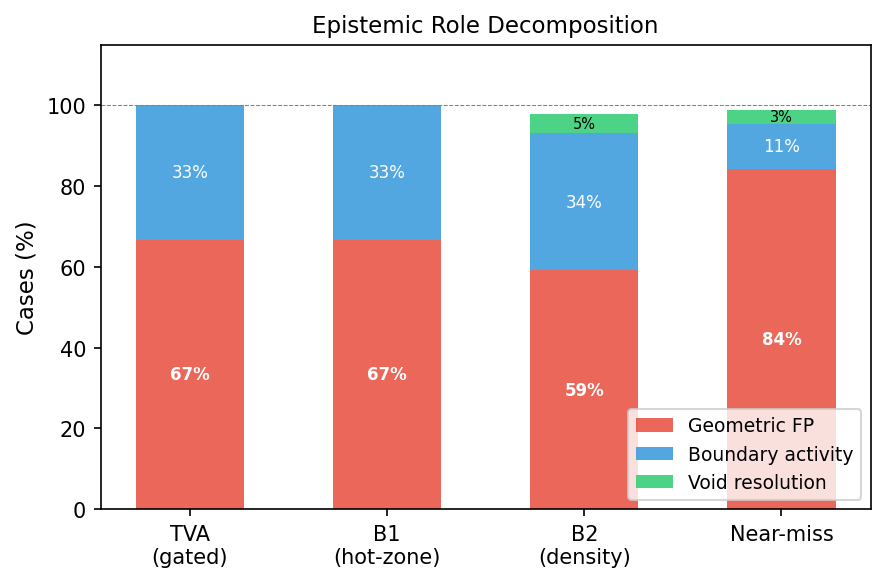
\includegraphics[width=\columnwidth]{figures/fig1_role_decomposition.png}
\caption{Epistemic role decomposition by source group (t3+t4+t5, n=1076 total).
Most raw fills are geometric false positives. Near-miss controls show the highest FP rate.}
\end{figure}

\subsection{Landmark Three-Layer Diagnostic}

As a positive-control diagnostic, we select five landmark bridge-type papers
(pre-specified, widely cited, 2019--2023) and apply the full three-layer TVV
predicate: geometric closure (G), anchor eligibility (E), and LLM-assisted bridge
interpretability audit (R). Each landmark uses its publication-year cutoff as the
train corpus boundary.

\begin{table}[h!]
\centering\small
\caption{Landmark three-layer diagnostic. All five papers clear G and E; none clear R.}
\resizebox{\columnwidth}{!}{%
\begin{tabular}{lcccc}
\toprule
Landmark & G & E & R \\
\midrule
vLLM / PagedAttention (2023) & \textbf{Yes} & \textbf{Yes} & No \\
MLIR (2020)                  & \textbf{Yes} & \textbf{Yes} & No \\
Devign (2019)                & \textbf{Yes} & \textbf{Yes} & No \\
Ansor (2020)                 & \textbf{Yes} & \textbf{Yes} & Weak \\
FlashAttention (2022)        & \textbf{Yes} & \textbf{Yes} & No \\
\bottomrule
\end{tabular}%
}
\end{table}

All five landmarks exceed the same-anchor null midpoint $p_{95}$ threshold (G~pass)
and are anchor-eligible for at least one TVA anchor (E~pass). However, LLM bridge
audit (R) finds that the corresponding best-void source pairs are semantically
incoherent: for example, vLLM's best void pairs a GPU energy survey with a VANET
routing paper, not OS paging with LLM serving.

This 5/5 G+E pass, 0/5 R pass pattern is precisely the failure mode TVV is designed
to surface. It demonstrates that the three layers are not redundant: geometric
proximity and anchor alignment are necessary screening signals but are insufficient
without role-aware interpretation. The detector beeps at the right domain, but
recovering the correct bridge pair requires the full adjudication pipeline.

\subsection{Finding 4: Geometric Impossibility of R-Layer Substitution}
\label{sec:finding4}

We tested whether the LLM-based R layer can be replaced by a closed-form
graph-spectral surrogate. Three independent operators were evaluated on the same
C1-restricted void population (Table~\ref{tab:spectral}).

\begin{table}[h!]
\centering\small
\caption{Three spectral surrogates for the R layer. All fail by distinct mechanisms.
NM = non-monotone rate (signal direction wrong).
\dag\,Degenerate (constant signal): $\kappa$ not meaningful.}
\label{tab:spectral}
\resizebox{\columnwidth}{!}{%
\begin{tabular}{llrrcc}
\toprule
Stage & Operator & $N$ & $\Delta$-signal & NM & $\kappa$ \\
\midrule
A & $\Delta R$ global & 51k & $0$ & --- & $-1.0$\dag \\
B & $\Delta R$ local & $\sim$328 & $9e{-}4$ & 74\% & $-0.013$ \\
C & $\Delta\kappa_\mathrm{ORC}$ & $\sim$329 & $2.4e{-}3$ & 43\% & $0.005$ \\
3a-Q1 & XEnc anchor & 100 & --- & --- & 0.10 \\
3a-Q2 & XEnc A+B & 100 & --- & --- & 0.01 \\
\bottomrule
\end{tabular}%
}
\end{table}

Stages B and C additionally share consistent weak negative Pearson
correlations with LLM fill labels ($r\approx -0.12$, both $p>0.20$),
suggesting a sub-threshold geometric signal whose signal-to-noise ratio
is insufficient for class adjudication under any tested operator.

\paragraph{Stage A: Global k-NN graph (N=51\,460).}
We computed the change in effective resistance $\Delta R/R_\mathrm{before}$ between
A- and B-side communities before and after inserting candidate filler $P$ into the
full BGE-M3 train corpus k-NN graph.
$\Delta R/R = 0.0000$ at machine precision across all 100 tested cases.
Cohen's $\kappa = -1.0$ vs LLM labels (degenerate: signal is a constant).
Root cause: in BGE-M3's anisotropic 1024-dimensional space, the global k-NN graph is
nearly fully connected, leaving no detectable resistance contrast.

\paragraph{Stage B: Localized subgraph (N$\approx$328).}
We restricted the graph to the C1 anchor pool plus $k$-NN neighborhoods of A, B,
and the midpoint (N$\approx$328, well within the regime where von Luxburg's
commute-time collapse should not apply).
$\Delta R/R$ showed a non-zero but uninformative distribution
(mean $= 9 \times 10^{-4}$, p50 $= 6 \times 10^{-4}$, p90 $= 3 \times 10^{-3}$).
Critically, 74\% of cases showed $\Delta R > 0$ (resistance \emph{increased}
after P was inserted), indicating non-monotone behavior: new nodes change the
degree distribution of both endpoints, and $\Delta R$ can be negative for true
bridges and positive for false positives (a network-level Braess-paradox effect).
Cohen's $\kappa = -0.013$ vs LLM labels, and Pearson $r(\Delta R, \mathrm{fill}) = -0.13$
($p = 0.21$). The signal is structurally noise.

\paragraph{Stage C: ORC path curvature (N$\approx$329, n=30).}
We tested Ollivier-Ricci curvature (ORC) on the same localized subgraph.
For each void, we computed mean ORC along the A$\to$B shortest path before and after
inserting $P$, recording $\Delta\kappa_\mathrm{path}$.
$\Delta\kappa$ showed a distribution with mean $2.4\times10^{-3}$ (p50 $=-3.0\times10^{-3}$,
p90 $=2.6\times10^{-2}$); 43\% of cases showed positive $\Delta\kappa$ (analogous to
the non-monotone pattern in Stage B).
Cohen's $\kappa = 0.005$ vs LLM labels; Pearson $r(\Delta\kappa, \mathrm{fill}) = -0.11$
($p = 0.57$). ORC path curvature shows no class-discriminative signal.

\paragraph{Stage 3a: Cross-Encoder Reranking.}
To test whether the impossibility extends beyond bi-encoder geometry, we evaluated
BGE-M3's own cross-encoder sibling (\texttt{bge-reranker-v2-m3}) on the same 100 cases.
The cross-encoder can attend to token-level interactions and thus bypasses the
bi-encoder bottleneck. Four query formats were tested: (Q1)~anchor text, (Q2)~A+B
concatenated, (Q3)~an explicit bridging prompt, (Q4)~min(score(P,A), score(P,B)).

Q1 (anchor) achieves AUC=0.875, confirming the cross-encoder detects anchor
relevance (G layer). However, Q2 (joint bridging) achieves AUC=0.352 $<$ 0.5 ---
\emph{anti-correlated} with fill. Inspecting the 4-class breakdown, INCREMENTAL-EXTENSION
and SURVEY-OR-NAMING papers score \emph{higher} on Q2 than PARTIAL-FILL papers
(means 0.17/0.19 vs.\ 0.018), because both are topically related to A or B but only
one side. The cross-encoder rewards single-domain proximity, not epistemic bridging.

Cohen's $\kappa = 0.010$ (Q2), 0.102 (Q1), 0.067 (Q3), $-0.014$ (Q4). No query format
reliably discriminates fill from non-fill. Cross-encoder reranking is the 4th
independent method to fail.

\paragraph{Synthesis and Impossibility Conjecture.}
Four independent methods fail across two inference paradigms (geometric operators
on Stages A--C, cross-encoder joint attention on Stage 3a) and four failure modes:
anisotropy collapse (Stage A), non-monotone sign instability (Stage B), flat
curvature (Stage C), and anti-correlated relevance (Stage 3a-Q2).
The consistency of failure across inference paths sharing the same BGE-M3 backbone
suggests the bridging signal is absent at the representation level, not merely at
the bi-encoder readout.

\begin{quote}\small
\emph{Conjecture (Architectural Impossibility).}
For retrieval-trained dense encoders under InfoNCE-class objectives,
$I(\text{geometric/attention features};\,R\mid\phi) \approx 0$
for cross-domain epistemic bridging within C1-restricted anchor pools.
This conjecture is grounded in four independent failures with distinct failure
modes, ruling out a single-operator explanation. Scope: C2/C3/C4 contribute
$\leq$7\% marginal selectivity on random pairs (Diagnostic~1); tighter
calibration may alter the void population but is unlikely to rescue
spectral surrogates given BGE-M3 anisotropy. Formal upper bounds on $I$
for arbitrary operator families require adversarial construction and are
left to future work.
\end{quote}

\paragraph{Implication.}
The R layer's reliance on text-level semantic assessment is a structural
necessity imposed by the architecture of contrastive bi-encoders.
The TVV three-layer design (G$\to$E$\to$R) reflects this asymmetry: geometric
layers are computationally cheap and architecturally captured by retrieval
encoders, while epistemic role requires inference beyond fixed-vector compression.

\subsection{Case Studies}

The following three cases are selected from the t4/t5 role audit to illustrate
why geometric proximity alone does not determine epistemic role.
For each case we report the anchor direction, the two source-side communities,
why the future paper is geometrically close, and why the role differs.

\paragraph{Case 1 -- Partial Fill~\cite{case1} (2019).}
Anchor: virtualization and cloud resource management.
Source~A lies on the VM resource allocation side; Source~B lies on
vehicular task-scheduling. The future paper studies multi-task offloading
over vehicular clouds, combining resource allocation, task scheduling,
and cloud/edge execution. Its embedding falls near the midpoint
($\mathrm{sim}(P,m){=}0.835$) because it shares vocabulary from both sides.
However, its reference list contains 10+ task-offloading citations (B-side)
but only one marginal VM reference (A-side).
It approaches the bridge but does not fully connect both source communities.
Role: PARTIAL-FILL.

\paragraph{Case 2 -- Boundary Expansion~\cite{case2} (2021).}
Anchor: kernel scheduling and CPU affinity for heterogeneous systems.
Source~A represents the kernel-scheduler/CPU-affinity side; Source~B represents
heterogeneous-system optimization. The future paper proposes AI planning heuristics
for heterogeneous HPC configuration and is geometrically close to the midpoint
($\mathrm{sim}(P,m){=}0.855$) through shared language of scheduling, planning,
and resource optimization.
Its entire bibliography (44 references) remains within the HPC optimization
literature; there are no kernel scheduler, CPU-affinity, or OS-level references.
It extends Source~B's direction without crossing toward Source~A.
Role: INCREMENTAL-EXTENSION.

\paragraph{Case 3 -- False Positive~\cite{case3} (2017).}
Anchor: storage I/O path optimization and NVMe driver design.
Despite having the \emph{highest} midpoint similarity of the three cases
($\mathrm{sim}(P,m){=}0.875$), the paper studies energy-aware virtual network
embedding. The high similarity is driven by generic vocabulary---``virtual'',
``resource'', ``energy'', ``allocation''---shared with cloud infrastructure papers
on both source sides, not by substantive connection to storage or NVMe research.
Its 19 references contain no storage I/O, NVMe, block-layer, or anchor-domain
citations. It is geometrically close but epistemically off-target.
Role: FALSE-POSITIVE.

\begin{figure}[h!]
\centering
\resizebox{\columnwidth}{!}{%
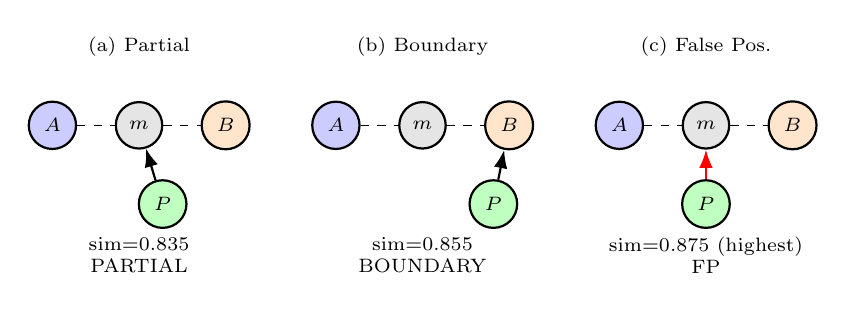
\begin{tikzpicture}[
  nd/.style={circle,draw,thick,minimum size=5.5mm,font=\scriptsize},
  lbl/.style={font=\scriptsize},
  ar/.style={-Latex,thick}
]
% Panel (a): Partial Fill  sim=0.835
\node[lbl] at (0,2.2) {(a) Partial};
\node[nd,fill=blue!20]  (Aa) at (-1.1,1.2) {$A$};
\node[nd,fill=orange!20](Ba) at ( 1.1,1.2) {$B$};
\node[nd,fill=gray!20]  (ma) at ( 0,  1.2) {$m$};
\node[nd,fill=green!25] (Pa) at ( 0.3,0.2) {$P$};
\draw[dashed] (Aa)--(ma)--(Ba);
\draw[ar] (Pa)--(ma);
\node[lbl,align=center] at (0,-0.45) {sim=0.835\\PARTIAL};

% Panel (b): Boundary Expansion  sim=0.855
\node[lbl] at (3.6,2.2) {(b) Boundary};
\node[nd,fill=blue!20]  (Ab) at (2.5,1.2) {$A$};
\node[nd,fill=orange!20](Bb) at (4.7,1.2) {$B$};
\node[nd,fill=gray!20]  (mb) at (3.6,1.2) {$m$};
\node[nd,fill=green!25] (Pb) at (4.5,0.2) {$P$};
\draw[dashed] (Ab)--(mb)--(Bb);
\draw[ar] (Pb)--(Bb);
\node[lbl,align=center] at (3.6,-0.45) {sim=0.855\\BOUNDARY};

% Panel (c): False Positive  sim=0.875
\node[lbl] at (7.2,2.2) {(c) False Pos.};
\node[nd,fill=blue!20]  (Ac) at (6.1,1.2) {$A$};
\node[nd,fill=orange!20](Bc) at (8.3,1.2) {$B$};
\node[nd,fill=gray!20]  (mc) at (7.2,1.2) {$m$};
\node[nd,fill=green!25] (Pc) at (7.2,0.2) {$P$};
\draw[dashed] (Ac)--(mc)--(Bc);
\draw[ar,red] (Pc)--(mc);
\node[lbl,align=center] at (7.2,-0.45) {sim=0.875 (highest)\\FP};
\end{tikzpicture}%
}% end resizebox
\caption{Case-study role patterns. Case~(c) has the \emph{highest}
$\mathrm{sim}(P,m)$ yet is a false positive; Case~(a) has lower similarity
but partially bridges both source sides. Geometric proximity alone does not
determine epistemic role.}
\label{fig:cases}
\end{figure}

\begin{figure}[h!]
\centering
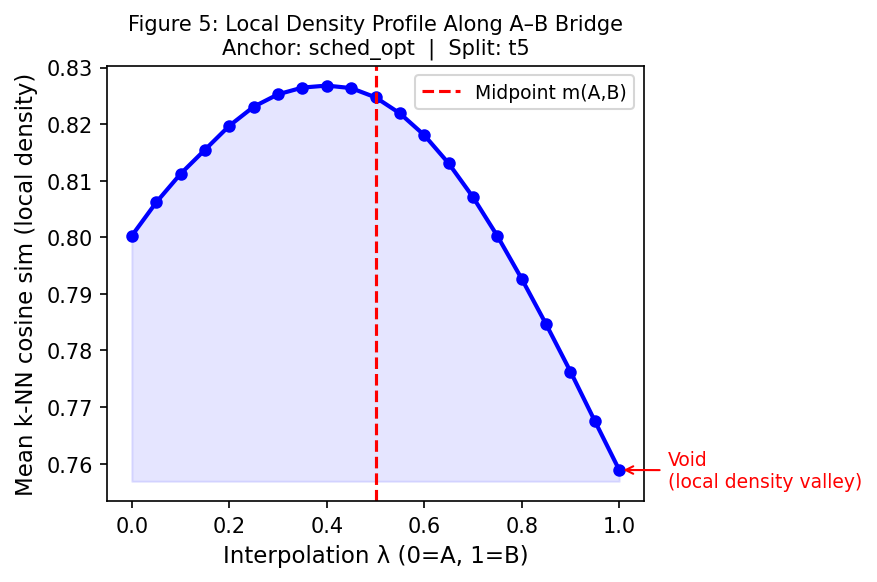
\includegraphics[width=\columnwidth]{figures/fig5_void_valley.png}
\caption{Local density profile along the A--B bridge for the highest-MMR void
in anchor sched\_opt (t5). The density valley at $\lambda\approx 0.5$ marks
the void midpoint region---two dense source communities with a less-occupied bridge.}
\end{figure}

\section{Discussion}

\subsection{Raw Fill Fails for Three Reasons}

Raw fill conflates void quality with sociotechnical realization rate:
(1)~hot-zone baselines are biased by local momentum;
(2)~fixed thresholds are not portable across anchor-density regimes;
(3)~anchor-eligible future papers are sparse ($\sim$6\%), right-censoring many unfilled voids.

\subsection{B2 Is a Control, Not a Competitor}

B2 is a strong counterfactual rather than a weak random baseline: it fixes the anchor
and matches local midpoint density, estimating the background rate at which future
literature occupies comparable regions without \tva{}'s structured void-selection criteria
(C1--C4).

Under calibrated thresholds, \tva{} reaches parity with B2 but does not outperform it.
We interpret this as a conservative result in a low-base-rate, corpus-limited regime: fill
events are rare, both methods are exposed to the same small set of future papers, and the
current corpus and validation windows may lack the statistical power to distinguish
structured void discovery from density-matched background occupancy.

Parity with B2 is in fact the expected outcome under a properly controlled design.
B2 matches the anchor and local density of \tva{} voids, so it estimates the background
arrival rate of future papers in comparable regions.
A large \tva{} advantage under this control would imply either strong method-specific
predictive signal or residual confounding; we observe neither.
Instead, both methods converge to the same low calibrated fill rate, indicating that
significant geometric closure is primarily base-rate limited in this corpus.

B2 is intentionally conservative: it makes raw-fill superiority difficult to claim
without evidence of signal beyond anchor and density.
\tva{} does not provide that signal at this scale---but it was not designed to win
on fill rate. Its value lies in turning a latent region into a named, inspectable,
and actionable ex-ante hypothesis $(A,B,q,m)$ before any future paper exists.
Raw temporal fill rate is not a sensitive metric for that kind of value.

\subsection{Why the R Layer Requires Language Models}

Our empirical impossibility result (Finding~4) has a natural theoretical grounding
in the form-meaning distinction articulated by \cite{bender2020climbing}:
\emph{"A system trained only on form has a priori no way to learn meaning."}
Dense retrieval encoders such as BGE-M3 are trained on form-form alignment:
they optimize whether two symbol sequences co-occur in relevance-annotated pairs.
This is sufficient for topical similarity (G layer, Stage 3a Q1 AUC$=0.875$) but
structurally insufficient for adjudicating communicative intent --- whether a
document's authors synthesize two research traditions rather than merely cite them.
This limitation is consistent with work showing that contrastive uniformity forces
distinct classes into maximally separated spherical caps~\cite{wang2020understanding},
and that form-trained dual-encoders fail on compositional benchmarks where surface
statistics are insufficient~\cite{mccoy2019right}.

The key distinction is \emph{compositionality} \cite{fodor1988connectionism} rather
than dimensionality. Bi-encoders compress each paper into a single fixed-length vector,
discarding compositional structure (P uses B's method to address A's problem).
Cross-encoders add joint attention but still collapse to a scalar readout; the
bridging signal is lost at that final compression (Stage 3a Q2 AUC$=0.352$,
anti-correlated with fill). Language models preserve the full token sequence and can
\emph{dynamically recompose} A- and B-side concepts during inference.
The R layer does not require an LLM because bridging is somehow ``in a higher
dimension''~--- it requires an LLM because bridging is a relational, compositional
property that fixed-vector compression discards.

The Q1 vs Q2 AUC gap on the cross-encoder (0.875 $\to$ 0.352) provides direct
empirical evidence of this gap: the encoder can rank by form-level proximity
(Q1), but negatively ranks by compositional synthesis (Q2).

\subsection{TVA as a Rapid Triage Instrument}

The absence of a significant TVA--B2 fill-rate advantage should not be interpreted
as an absence of practical utility. B2 is a strong \emph{retrospective control}, not
a discovery workflow: it estimates how often density-conditioned regions receive future
occupancy. TVA, by contrast, produces a ranked list of inspectable void hypotheses
$(q,A,B,m)$ within minutes. Parity with B2 under dependence-aware tests is therefore
nontrivial: TVA reaches the background future-occupancy rate of a strong matched
control while also providing human-readable source-side structure for follow-up.

TVA is a \emph{detector}, not an oracle. A high TVA signal is analogous to an anomaly
reading: it prioritizes candidate locations for inspection, but does not certify
epistemic closure. TVV provides the downstream adjudication protocol---calibrated
geometric closure, anchor observability, and role-aware assessment---to determine
whether a candidate void corresponds to a genuine epistemic gap.

\paragraph{Human-machine division of labor.}
The combinatorial search for candidate voids is machine-scale: a modest anchor
neighborhood of 300 source papers induces ~45\,000 candidate pairs, and TVA
generates 300 ranked void hypotheses across 10 anchors in minutes. Human experts
are not designed for exhaustive enumeration at this scale, but are well-suited to
adjudicating a compact, ranked list of interpretable $(q,A,B,m)$ candidates.
TVA therefore functions as a high-throughput triage step that compresses a
machine-scale search space to a human-auditable hypothesis set.

\begin{table}[h!]
\centering\small
\caption{Division of labor.}
\resizebox{\columnwidth}{!}{%
\begin{tabular}{lll}
\toprule
Task & Human & TVA/TVV \\
\midrule
Enumerate pairs & Infeasible & Automatic \\
Rank voids & Infeasible & Automatic \\
Anchor alignment & Difficult & Automatic \\
Bridge meaning & Strong & Assisted \\
Technical merit & Strong & Exploratory \\
\bottomrule
\end{tabular}%
}
\end{table}

\tva{} should therefore be evaluated as a \emph{rare-event triage instrument}.
Because genuine epistemic closure is a low-base-rate event, most candidate voids will
not become validated closures within any finite corpus window. The relevant measure is
not absolute conversion rate but \emph{enrichment}: does TVA concentrate observable
future-bridging events into a smaller, inspectable candidate set relative to unguided
or density-only search? Three rates matter at distinct levels: (i)~\emph{detection
rate}---does TVA surface the right anchor domain? (ii)~\emph{interpretability rate}---does
the A/B/q hypothesis make structural sense? and (iii)~\emph{realization rate}---does
a future paper actually close the predicted gap? Only the first two are directly
measurable from pre-publication corpora; realization is what TVV attempts to
evaluate, and it is expectedly rare.

\noindent\emph{Note}: TVA produces $(q,A,B,m)$ hypotheses for downstream review;
B2 produces matched midpoints to estimate background occupancy. The two serve
fundamentally different roles and are not competing discovery systems.

\subsection{From Geometric Occupancy to Role Decomposition}

Future papers near void midpoints decompose into true fills, boundary expansions, and
false positives. The scarcity of true fills reveals that genuine epistemic closure is
a much stricter condition than geometric occupancy.
\emph{The three layers are operational screens for disentangling three sources of
evidence that raw fill rate conflates: geometric occupancy, observability, and
epistemic role. They are not claimed to be necessary and sufficient conditions
for scientific discovery.}

\subsection{Descriptive, Not Evaluative}

\tvv{} classifies the type of validation evidence produced by future literature, not
the intrinsic merit of papers. Boundary expansion and incremental extension are
valuable scientific activities.

\subsection{Dynamic Extension (Future Work)}

The static-snapshot design of \tvv{} evaluates fill outcomes at a fixed
time horizon. A natural extension is to evaluate void evolution
continuously as new papers arrive. We leave the formalization and
empirical study of such dynamic protocols to future work.

\subsection{Threats to Validity}

(1)~\emph{Embedding dependence}: all metrics use BGE-M3.
(2)~\emph{Threshold sensitivity}: calibration uses 200 null midpoints per cell.
(3)~\emph{Corpus coverage}: fills outside arXiv are unobservable; unfilled voids are right-censored.
(4)~\emph{LLM classification reliability}: role labels are produced by a single LLM
(Claude Sonnet~4.5) using a fixed rubric. To assess reliability: (i)~blind
source-label removal (source group not shown to classifier); (ii)~cross-LLM
re-annotation on 100 stratified t5 cases (Claude~4.5 vs.\ GPT-5.2;
$\kappa_3{=}0.44$, ``moderate''; see §4.3); (iii)~a blinded human audit on
60 cases ($>$80\% binary FP agreement, $\sim$65\% 3-class). Epistemic role is
inherently interpretive; neither cross-LLM nor human labels constitute ground truth.
(5)~\emph{Domain specificity}: CS arXiv categories only.
(6)~\emph{Encoder generality}: the architectural impossibility result is established
on BGE-M3 and its cross-encoder sibling. Replication on E5, GTE, or
instruction-tuned encoders is left to future work.
(7)~\emph{Calibration and inference assumptions}. The null calibration in §4.1
assumes exchangeability of null midpoints within anchor-density cells; we argue
informally based on the stratified sampling construction, but do not provide a
formal identification proof. Multiplicity across the four geometric impossibility
stages (A/B/C/3a) is not explicitly corrected; under Bonferroni at $m{=}4$, all
qualitative conclusions are unchanged given the magnitude of null results
($|\kappa|{\leq}0.01$). Anchor-level clustering is addressed via hierarchical
bootstrap (10 anchors as primary resampling unit,
$\widehat{\mathrm{ICC}}{\approx}0.87$, $n_\mathrm{eff}{\approx}11$); finer-grained
random-effects modelling is left to future work.

\section{Related Work}

\textbf{Validation of Predicted Voids.}
Prior retrospective evaluations in LBD~\cite{swanson1986fish,gordon1996using,weeber2001using}
typically validate predicted connections by checking whether future publications instantiate
an A--B association. Knowledge-graph completion similarly evaluates whether missing edges
are recoverable under a fixed relation schema. These settings differ from void validation:
a \tva{} void is not a predicted edge but an anchor-conditioned geometric vacancy whose
future occupancy may represent true bridging, boundary expansion, or false-positive
proximity. To our knowledge, prior work has not evaluated embedding-space voids under
density-controlled, observability-aware, and role-aware temporal validation. \tvv{}
addresses this gap.

\textbf{Literature-Based Discovery.}
Swanson's ABC model~\cite{swanson1986fish} and subsequent LBD work~\cite{gordon1996using,weeber2001using} validate predictions by checking future
publication appearance. \tvv{} extends this tradition by requiring epistemic bridging
role, not merely geometric proximity.

\textbf{Novelty and First-Story Detection.}
Topic Detection and Tracking~\cite{allan1998topic} introduced first-story detection; novelty detection in IR~\cite{zhang2002novelty}
measures whether a document adds new information relative to a query set. Our
first-filler intuition shares the event-ordering structure but operates on knowledge
structure rather than event reporting.

\textbf{Structural Holes and Scientometrics.}
Burt's structural hole theory~\cite{burt2004structural} shows brokers spanning gaps accumulate informational
advantage. Co-citation analysis~\cite{small1973cocitation} and our density-matched baseline directly control for hot-zone momentum.

\textbf{Dense-Region Bias in Embeddings.}
Anisotropy in high-dimensional text embeddings~\cite{ethayarajh2019contextual} compresses cosine similarities into a
narrow range. We show this anisotropy makes fixed thresholds non-portable in
downstream void validation. Our use of ``topological'' is operational rather than
homological~\cite{carlsson2009topology,edelsbrunner2010computational}.

\textbf{Scientific Claim Verification.}
Epistemic classification of scientific contributions---argumentative zoning~\cite{teufel2002summarizing},
overclaiming detection~\cite{wright2022generating}---provides precedents for our role-aware rubric. \cite{wadden2020scifact} introduced scientific fact verification as a retrieval task; our R layer extends this from claim-level verification (does evidence support a claim?) to bridge-level role assessment (does P bridge A and B under anchor q?). The form-meaning gap articulated by \cite{bender2020climbing} provides the theoretical backdrop for our architectural impossibility result (\S\ref{sec:finding4}).

\section{Conclusion}

Temporal validation of predicted research voids requires separating geometric occupancy,
density bias, anchor observability, and epistemic role.
Under density matching, \tva{}'s apparent disadvantage disappears but is not
statistically significant. Under null-calibrated thresholds, fill rates collapse to
$\sim$0.7\%---most raw fills were null-zone noise.
LLM-assisted role-aware classification suggests that genuine epistemic bridging is rare even among
geometrically close, anchor-eligible future papers.

We propose a three-layer validation framework and leave two open questions for future
work: (1)~scalable role-aware validation without prohibitive LLM cost;
(2)~dynamic event-driven extensions in which each arriving paper updates knowledge-space
state.

\bibliographystyle{plain}
\bibliography{paper2}

\newpage
\appendix

\section{Reproducibility Protocol}
\label{app:protocol}

\paragraph{Corpus.}
arXiv metadata (title, abstract, categories, update\_date) for categories
cs.OS, cs.AR, cs.PL, cs.SE, cs.DC, cs.NI, cs.CR, cs.AI, cs.LG.
Filtered by category; year assigned from update\_date.

\paragraph{Temporal splits.}
Three non-overlapping splits. For split $s$ with cutoff $T_s$:
train = papers with year $< T_s$; val = papers with year $\in [T_s, T_s+5)$.

\begin{table}[h]
\centering\small
\caption{Temporal split parameters. $N$ approximate; exact t5 train $N{=}51{,}460$.}
\resizebox{\columnwidth}{!}{%
\begin{tabular}{llllll}
\toprule
Split & Train end & Val window & Train $N$ & Val $N$ & Seed \\
\midrule
t3 & 2014-12-31 & 2015--2019 & $\sim$29k & $\sim$101k & 42 \\
t4 & 2016-12-31 & 2017--2021 & $\sim$35k & $\sim$171k & 42 \\
t5 & 2018-12-31 & 2019--2023 & $\sim$51k & $\sim$193k & 42 \\
\bottomrule
\end{tabular}%
}
\end{table}

\paragraph{Embedding.}
BGE-M3 (BAAI/bge-m3, 1024-dimensional, cosine similarity, offline/local mode).
Papers embedded as ``\textit{title} \textit{abstract}'' concatenation.

\paragraph{TVA void generation.}
For each anchor $q$ in Table~\ref{tab:anchors} and each split:
(1)~embed anchor text with BGE-M3;
(2)~retrieve top-300 cosine-nearest train papers (C1 pool);
(3)~enumerate all pairs and apply C1--C4 conditions;
(4)~rank by MMR score and output top-30 voids.
No anchor added or removed after validation runs began.

\begin{table}[h]
\centering\small
\caption{TVA anchor list (pre-specified, fixed across all splits).}
\label{tab:anchors}
\resizebox{\columnwidth}{!}{%
\begin{tabular}{ll}
\toprule
Key & Anchor phrase \\
\midrule
sched\_opt & kernel scheduler optimization and CPU affinity for multicore systems \\
mm\_vm & virtual memory management and page reclamation in operating systems \\
ebpf\_obs & eBPF programs for kernel tracing and system call observability \\
hwsw\_x86 & hardware-software co-design for x86 processor microarchitecture \\
net\_io & high-performance network I/O and packet processing in the kernel \\
sync\_lock & synchronization primitives and lock-free data structures \\
mem\_alloc & memory allocator design and heap fragmentation in systems software \\
virt\_hyp & virtualization and hypervisor design for cloud workloads \\
power\_mgmt & dynamic power management and CPU frequency scaling \\
storage\_io & storage I/O path optimization and NVMe device drivers \\
\bottomrule
\end{tabular}%
}
\end{table}

\paragraph{B1 baseline.}
For each anchor, sample 20 random pairs without replacement from the C1 pool
(seed 42). No void conditions applied.

\paragraph{B2 density-matched baseline.}
For each TVA void $V$, compute midpoint density $\rho(m_V)$ (mean cosine
similarity to $k{=}20$ nearest train neighbors). Sample 300 B1-style pairs
from the same anchor's C1 pool (seed 99). Select the pair whose midpoint
density is closest to $\rho(m_V)$ as the B2 counterpart.

\paragraph{Local density.}
\[\rho(m) = \frac{1}{k}\sum_{i=1}^{k}\mathrm{sim}(m, \mathrm{kNN}_i(m)),\quad k{=}20.\]

\paragraph{Anchor-eligibility threshold.}
$\tauanchor = \max(Q_{80}^{\mathrm{val}},\, Q_{90}^{\mathrm{train}})$,
computed per anchor and split.

\paragraph{Null-calibrated threshold.}
For each cell (anchor $q$, density bucket $b \in \{$low, mid, high$\}$, split $t$):
(1)~generate $n{=}1000$ null midpoints from C1 pool;
(2)~split 50/50 calibration/held-out;
(3)~compute $Z(m_0) = \max_{P \in \mathrm{Val}_q}\mathrm{sim}(P,m_0)$ for each null;
(4)~$\taufill = s_{(k)}$ where $k = \lceil(n_\mathrm{cal}+1)(1-\alpha)\rceil$
(finite-sample conformal quantile), $\alpha{=}0.05$.

\paragraph{Statistical tests.}
Primary inference uses \emph{hierarchical cluster bootstrap} (outer: resample anchors
with replacement; inner: resample voids within each anchor) for TVA--B2 difference in
percentage points. Secondary check: \emph{anchor-level sign-flip permutation test}
(randomly flip sign of per-anchor mean TVA--B2 difference; $n_\mathrm{perm}{=}10000$).
Both report two-sided $p$-values.

\paragraph{Role annotation.}
Model: Claude Sonnet~4.5, temperature~0.1.
Input: anchor text, source A title+abstract (truncated), source B title+abstract,
candidate filler title+abstract.
Output: JSON with role label, confidence, and six ordinal scores.
Source group labels are not shown (blind classification).
Final labels use the collapsed three-class taxonomy (Table~\ref{tab:rubric}).
Prompt and full rubric text are available upon request.

\paragraph{Code and data availability.}
Experiment scripts, prompts, and configuration files are maintained in an
internal repository at Intel Corporation. They will be made available
upon publication subject to internal review and export control clearance.
Derived labels for the role-classified 1,076 cases will be released with the
camera-ready version.

\end{document}
